\documentclass{article}
\usepackage{cmap}					% поиск в PDF
\usepackage[T2A, T1]{fontenc}
\usepackage[utf8]{inputenc}
\usepackage[english, russian]{babel}
\usepackage{enumitem} %[label=\alph*)]]
%%% Работа с русским языком
\usepackage{mathtext} 				% русские буквы в формулах
\usepackage{ccfonts,eulervm,euler}
\usepackage{bbding}
\usepackage{ulem}
\usepackage{indentfirst}
\usepackage{hyperref} %гиперссылки
\frenchspacing

\usepackage{fancyhdr} %Для шапки
\usepackage{amsthm}
\usepackage{amsmath}
\usepackage{amssymb} % R, Q,.
\usepackage{mathtools}
\usepackage{multicol}

\usepackage{indentfirst}
\parindent=1cm
\setlist[itemize]{itemsep=2pt, topsep=0pt} %norm lists
\setlist[enumerate]{itemsep=2pt, topsep=0pt} %norm lists

%%% Страница
\usepackage{geometry} % Простой способ задавать поля
\geometry{top=25mm}
\geometry{bottom=20mm}
\geometry{left=20mm}
\geometry{right=20mm}


%Определение, теорема, лемма, N.B.
\newtheorem*{defin*}{Определение}
\newtheorem{defin}{Определение}
\newtheorem*{Corollary*}{Следствие}
\newtheorem{Corollary}{Следствие}
\newtheorem*{Lemma*}{Лемма}
\newtheorem{Lemma}{Лемма}
\newtheorem{Theorem}{Теорема}
\newtheorem*{Theorem*}{Теорема}
\newtheorem{NB}{N.B}
\newtheorem*{NB*}{N.B}
\newtheorem{Example}{Пример}
\newtheorem*{Example*}{Пример}

%Proof
\newenvironment{Proof}
{\par\noindent{\bf Доказательство.}} 
{\hfill$\scriptstyle\blacksquare$}

\newcommand{\eq}[1][m]{\mathop{\equiv}\limits_{#1}}

\newcommand{\smallheader}[1]{\noindent{\bf #1 }}

\newcommand{\divs}{\,\lower.4ex\vdots\,}% a делится на b

\newcommand{\rmy}[1][m]{\mathbb{R}^{#1}}%$R^m$

\newcommand{\eqdef}{\overset{def}{\underset{}{=}}}% =def

\newcommand{\shapka}[1]{\pagestyle{fancy}\fancyhead[C]{#1}\fancyfoot{}}%Шапка

\newcommand{\chast}[2]{\dfrac{\partial #1}{\partial #2}}

%TADA https://youtu.be/9Cq56iPTQ5A?t=20
\newcommand{\THEN}{\text{\href{https://youtu.be/9Cq56iPTQ5A?t=20}{Тогда }}}

\usepackage{listings}
\usepackage{xcolor}

%New colors defined below
\definecolor{codegreen}{rgb}{0,0.6,0}
\definecolor{codegray}{rgb}{0.5,0.5,0.5}
\definecolor{codepurple}{rgb}{0.58,0,0.82}
\definecolor{backcolour}{rgb}{0.95,0.95,0.92}

%Code listing style named "mystyle"
\lstdefinestyle{mystyle}{
	backgroundcolor=\color{backcolour},   commentstyle=\color{codegreen},
	keywordstyle=\color{magenta},
	numberstyle=\tiny\color{codegray},
	stringstyle=\color{codepurple},
	basicstyle=\ttfamily\footnotesize,
	breakatwhitespace=false,         
	breaklines=true,                 
	captionpos=b,                    
	keepspaces=true,                 
	numbers=left,                    
	numbersep=5pt,                  
	showspaces=false,                
	showstringspaces=false,
	showtabs=false,                  
	tabsize=2
}

\lstset{style=mystyle}

\title{Code Listing}


\begin{document}
	\shapka{Ашихмин Анатолий (M3239),  Клепов Дмитрий (M3238), Тарасов Егор (M3238)\\
	Обратная связь: dimkakirov43@mail.ru}
	{\bf Задача.}
	
	Для случайных величин выполнить следующие действия:
	\begin{itemize}
		\item Построить графики функций распределения
		\item Построить выборку и по ней график эмпирической функции распределения
		\item На  графике построить доверительную полосу для нее и  убедиться, что функция распределения попадает в полосу
		\item На основе критериев Колмогорова и Смирнова провести проверку гипотез
	\end{itemize}

	\begin{enumerate}
		\item {\bf Графики.}\\
		
		\begin{figure}[h]
			\centering
			\begin{minipage}{0.45\textwidth}
				\centering
				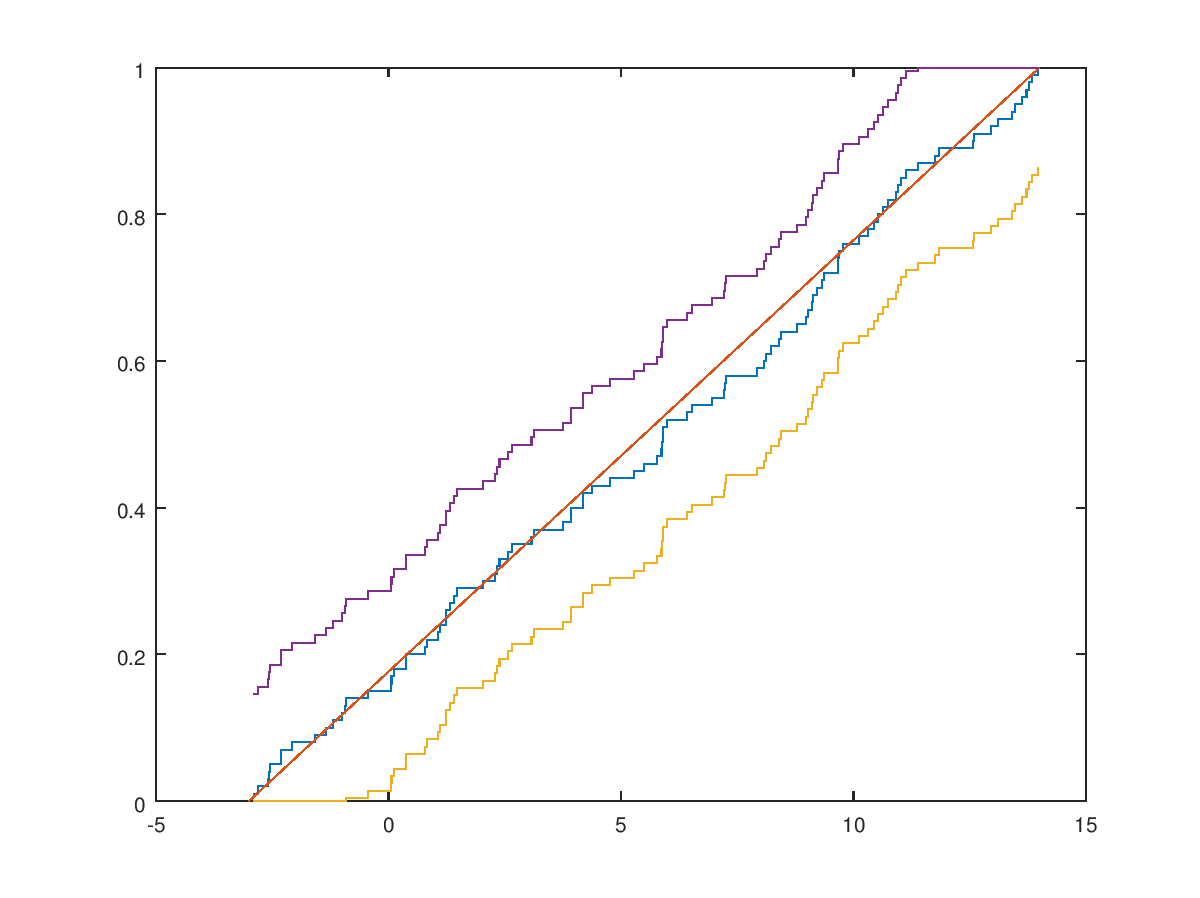
\includegraphics[width=\textwidth]{unif.png}
				\caption{Равномерное: $U_{-3,14}$}
			\end{minipage}\hfill
			\begin{minipage}{0.45\textwidth}
				\centering
				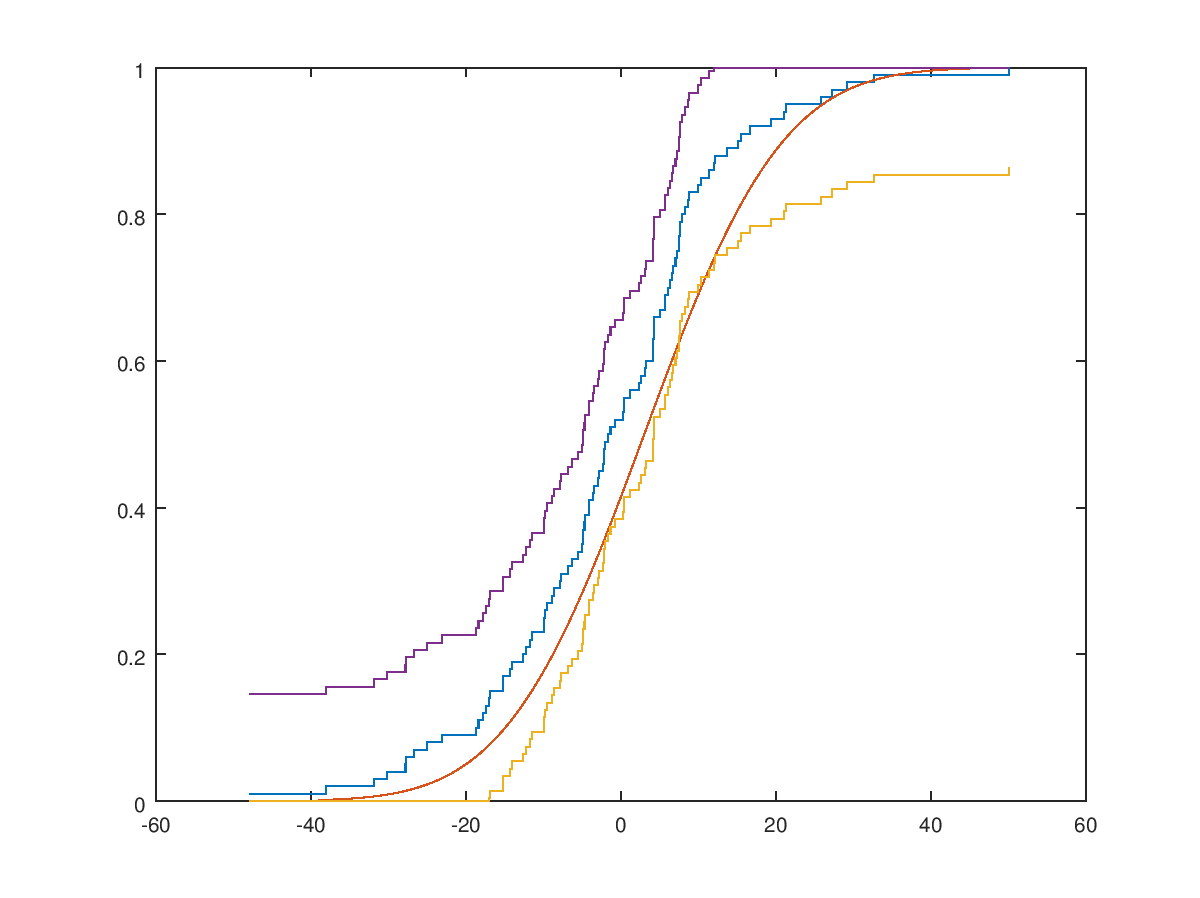
\includegraphics[width=\textwidth]{norm_plt.png} % second figure itself
				\caption{Нормальное: $N_{3,14}$}
			\end{minipage}
		\end{figure}
		
		\begin{itemize}
			\item Нормальное ($N_{3,14}$), код:
			\lstinputlisting[language=Octave]{norm_plt.m}

			\item Равномерное ($U_{-3,14}$), код:
			\lstinputlisting[language=Octave]{unif.m}
			
		\end{itemize}
		\item {\bf Тесты:}
		
		\begin{itemize}
			\item Нормальное
			\lstinputlisting[language=Octave]{norm_tests.m}
			
			{\bf Выход:}
			
			\begin{lstlisting}
Kolmogorov: n = 10000, alpha = 0.0455

Smirnov: n = 10000, alpha = 0.0488

Kolmogorov: n = 1000000, alpha = 0.044717

Smirnov: n = 1000000, alpha = 0.049323\end{lstlisting}
			
			\item Равномерное
			\lstinputlisting[language=Octave]{ravn_tests.m}
			
			{\bf Выход:}
			
			\begin{lstlisting}
Kolmogorov: n = 10000, alpha = 0.0447

Smirnov: n = 10000, alpha = 0.0508

Kolmogorov: n = 1000000, alpha = 0.044915

Smirnov: n = 1000000, alpha = 0.049568\end{lstlisting}
		\end{itemize}
		
		\item {\bf  Вывод:}
		
		Реальная функция распределения попала в доверительную полосу.\\
		Эмпирическая функция распределения является качественной оценкой функции распределения. Это подтверждается результатом тестов, проведенных на основе критерия Колмогорова и Смирнова.
		
	\end{enumerate}
\end{document}